\begin{pastexam}[label={px:df3-097-ds-01}]{地方三等資訊處理 97 年 第一題}
（申論；35 分）

heap sort 是一個有名的排序演算法。請回答下列問題：
\begin{enumerate}[leftmargin=2.6em, labelsep=0.4em]
\item[㈠] 下圖是 heap 的一個例子，請你說明何謂 heap？（5 分）
\begin{center}
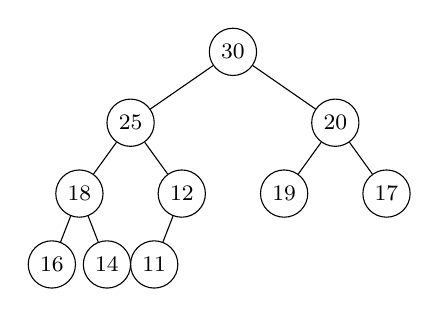
\begin{tikzpicture}[n/.style={circle,draw,inner sep=0pt,minimum size=6mm,font=\footnotesize},
  level distance=9mm, level 1/.style={sibling distance=26mm}, level 2/.style={sibling distance=13mm},
  level 3/.style={sibling distance=7mm}]
\node[n] {30}
  child {node[n] {25} child {node[n] {18} child {node[n] {16}} child {node[n] {14}}}
                      child {node[n] {12} child {node[n] {11}} child[missing]}}
  child {node[n] {20} child {node[n] {19}} child {node[n] {17}}};
\end{tikzpicture}
\end{center}
\item[㈡] heap sort 通常使用 heap 的樹狀示意圖（如上圖）來表示其執行的過程。但在實作 heap sort 的程式時，
我們通常並不使用二元樹（binary tree）的資料結構來存放其資料，而改採用另一種資料結構，請問是那一種
資料結構？它是如何存資料的？（5 分）
\item[㈢] 和 merge sort 比起來，heap sort 有何優點？（5 分）
\item[㈣] 和 quick sort 比起來，heap sort 有何優點？（5 分）
\item[㈤] heap sort 在排序 n 個資料時，其時間複雜度（time complexity）為何？（5 分）
\item[㈥] 如果輸入之資料中所有 n 個元素的值均相等，那麼請問 heap sort 的執行時間會不會變得比較快（和亂數
輸入的資料比起來）？還是變得比較慢？請說明理由。（5 分）
\item[㈦] heap sort 算是一個不錯的排序演算法，可惜它不是一個“stable”的 sort 方法。請你用較簡單的方法，將
heap sort 改良一下，將它變成一個“stable”的 sort 方法。（5 分）
\end{enumerate}
\end{pastexam}

\begin{pastsoln}
\textbf{㈠} heap（堆積）是滿足下面兩個條件的二元樹（資結書第~8.1~節）：
\begin{enumerate}[label=(\arabic*)]
\item \textbf{形狀}：是完整二元樹（complete binary tree），除了最後一層都是滿的，最後一層的節點靠左排。
\item \textbf{順序}：每個節點的值都大於或等於它的子節點的值（最大堆積，max-heap）。 反過來「小於或
等於」的叫最小堆積。
\end{enumerate}
由 (2)，根是全部裡最大的。 圖中的例子：$30 \ge 25, 20$；$25 \ge 18, 12$；$20 \ge 19, 17$；$18 \ge 16, 14$；
$12 \ge 11$，而且最後一層的 $16, 14, 11$ 由左往右排滿前三個位置，是一個最大堆積。 注意堆積只規定
父子之間的大小，兄弟之間、不同子樹之間沒有規定（例如 $19$ 在右子樹、$18$ 在左子樹，$19 > 18$ 沒有關係）。

\textbf{㈡} 用一維\textbf{陣列}（資結書第~7.2.1~節）。 完整二元樹由上到下、同一層由左到右編號
$1, 2, \ldots, n$，第 $i$ 號節點存在 $A[i]$，父子關係用下標算，不必存指標：
\[
\text{左子} = 2i, \qquad \text{右子} = 2i + 1, \qquad \text{父} = \lfloor i/2 \rfloor .
\]
完整二元樹的編號沒有空洞，所以陣列 $A[1..n]$ 剛好塞滿。 題目的堆積存成
\begin{center}
\small
\begin{tabular}{c|cccccccccc}
$i$ & 1 & 2 & 3 & 4 & 5 & 6 & 7 & 8 & 9 & 10 \\
\hline
$A[i]$ & 30 & 25 & 20 & 18 & 12 & 19 & 17 & 16 & 14 & 11 \\
\end{tabular}
\end{center}
例如 $A[2] = 25$ 的子是 $A[4] = 18$、$A[5] = 12$；$A[5] = 12$ 的左子是 $A[10] = 11$，右子 $A[11]$ 不存在。
堆積排序直接在待排序的陣列裡原地建堆、原地取出，不需要另外配置節點。 （下標從 $0$ 開始的 C 陣列，
公式改成 $2i + 1$、$2i + 2$、$\lfloor (i - 1)/2 \rfloor$。）

\textbf{㈢ 和 merge sort 比}。 兩者最壞都是 $O(n \log n)$。 heap sort 是\textbf{原地}排序，只用
$O(1)$ 的額外空間；陣列版的 merge sort 合併時需要 $\Theta(n)$ 的暫存陣列（資結書第~14.4~節）。
記憶體吃緊時 heap sort 較好。 （反過來，merge sort 是穩定的，而且循序存取，適合鏈結串列和外部排序。）

\textbf{㈣ 和 quick sort 比}。 quick sort 平均 $O(n \log n)$，但最壞 $\Theta(n^2)$（例如以第一個數為
基準、輸入已排好序，資結書第~14.5~節）；heap sort 的\textbf{最壞情況也是} $O(n \log n)$，有保證。
另外 heap sort 不用遞迴，額外空間 $O(1)$；quick sort 的遞迴堆疊平均 $O(\log n)$、最壞 $O(n)$。
（實務上 quick sort 的常數小、快取表現好，平均比 heap sort 快，這是 heap sort 的缺點。）

\textbf{㈤} $O(n \log n)$，最好、平均、最壞都是（資料不全相等時）。 建堆用由下而上的方法是 $O(n)$
（資結書定理~8.1）；接著做 $n - 1$ 次「把根換到最後、從根往下調整」，每次下沉最多走樹高
$\lfloor \lg n \rfloor$ 層，共 $O(n \log n)$。 對一般的輸入，下沉通常要走到接近底部，所以也是
$\Omega(n \log n)$，合起來 $\Theta(n \log n)$。

\textbf{㈥ 會變快}，變成 $\Theta(n)$。 理由在下沉（Sift-Down，資結書虛擬碼~8.1）的停止條件：先比較
兩個子節點找出較大的，再比較「父 $\ge$ 較大的子」成立就停。 所有值相等時，這個條件第一次就成立，
每次下沉最多 $2$ 次比較、不交換、不往下走。 所以：
\begin{itemize}
\item 建堆：$\lfloor n/2 \rfloor$ 次下沉，每次 $O(1)$，共 $O(n)$；
\item 取出階段：$n - 1$ 次「交換根和最後一個＋一次下沉」，每次 $O(1)$，共 $O(n)$。
\end{itemize}
總共 $\Theta(n)$，約 $3n$ 次比較；亂數輸入約 $2n \lg n$ 次比較（例如 $n = 10000$ 時，全相等約 $3$
萬次，亂數約 $23$ 萬次）。 這個結論依賴停止條件用「$\ge$」：若程式寫成「父 $>$ 子才停」，相等時
會一直交換到底，執行時間仍是 $\Theta(n \log n)$，和亂數輸入差不多，不會更慢。

\textbf{㈦ 改成穩定}。 最簡單的作法：把每個資料的\textbf{原始位置}當成第二個鍵。 第 $i$ 個資料
變成 $(\mathit{key}_i, i)$，比較時先比 $\mathit{key}$，相等再比 $i$：
\[
(k_1, i_1) < (k_2, i_2) \iff k_1 < k_2 \text{ 或 } (k_1 = k_2 \text{ 且 } i_1 < i_2) .
\]
這樣所有資料兩兩不同，heap sort 排出的順序唯一確定，而且相等的 $\mathit{key}$ 依原始位置由小到大
排，正是穩定排序的定義。 代價是每筆多存一個整數，額外空間 $\Theta(n)$，時間仍是 $O(n \log n)$
（比較變成兩步，常數倍）。 heap sort 本身不穩定的原因，是「把根換到陣列最後」會把相等的資料跨越很遠
地交換，例如 $\langle 5_a, 5_b \rangle$ 建堆後交換根與最後一格，排完變成 $\langle 5_b, 5_a\rangle$，
原本 $5_a$ 在前。 加上位置當第二鍵後，$(5, 2) > (5, 1)$，$5_b$ 被視為較大的，會被放在後面。
\end{pastsoln}
